\documentclass[]{report}
\usepackage{kotex}
\usepackage{verbatim} 
\usepackage{graphicx} 

\usepackage{listings}
\usepackage{color}

\definecolor{dkgreen}{rgb}{0,0.6,0}
\definecolor{gray}{rgb}{0.5,0.5,0.5}
\definecolor{mauve}{rgb}{0.58,0,0.82}

\lstset{frame=tb,
	language=Java,
	aboveskip=3mm,
	belowskip=3mm,
	showstringspaces=false,
	columns=flexible,
	basicstyle={\small\ttfamily},
	numbers=none,
	numberstyle=\tiny\color{gray},
	keywordstyle=\color{blue},
	commentstyle=\color{dkgreen},
	stringstyle=\color{mauve},
	breaklines=true,
	breakatwhitespace=true,
	tabsize=3
}


% Title Page
\title{HW01 - REPORT}
\author{정보컴퓨터공학부 201624536 이국현}


\begin{document}
\maketitle


\section{서론}

\begin{itemize}
	\item 이미지 표현 방법
	\item 이미지 함수
	\item 이미지 변환
\end{itemize}

\subsection{이미지}
컴퓨터에서 이미지를 표현할 때는 일반적으로 2차원 행렬의 픽셀로 표현한다. 각 픽셀은 컬러 이미지의 결우 RGB(256,256,256) 3byte의 값을 가지고 흑백 이미지의 경우 하나의 1byte 픽셀 값을 가진다.\\

\subsection{이미지 함수}

이미지는 위치 x, y에 대한 색상 값이라는 함수로도 표현할 수 있다. 


\begin{itemize}
	\item 흑백 이미지
\end{itemize}

\[ f: [a,b] \times [c,d] \rightarrow [0, 255] \]

\begin{itemize}
	\item 컬러 이미지
\end{itemize}

\[ f(x,y) = [r(x,y), g(x,y), b(x,y)] \] \\

\subsection{이미지 변환}


\[ g(x, y) = f(x, y) + 20 \]

흑백 이미지의 경우 각 픽셀에 값을 더하여 이미지를 전체적으로 밝게 변환할 수 있다.\\


\[ g(x, y) = f(-x, y)\]

원본 이미지의 픽셀 값을 y 축 대칭으로 교환하여 대칭 이동된 이미지를 얻을 수 있다.\\

\[ g(x, y) = f(x, y + 20)\]

마찬가지로 (x, y)에 대한 픽셀 값으로 (x, y + 20)의 픽셀 값을 가져와 아래로 평행 이동시킬 수 있다.\\ 

\section{본론}

\subsection{원본 이미지}

\begin{figure}[ht!]
	\centering
	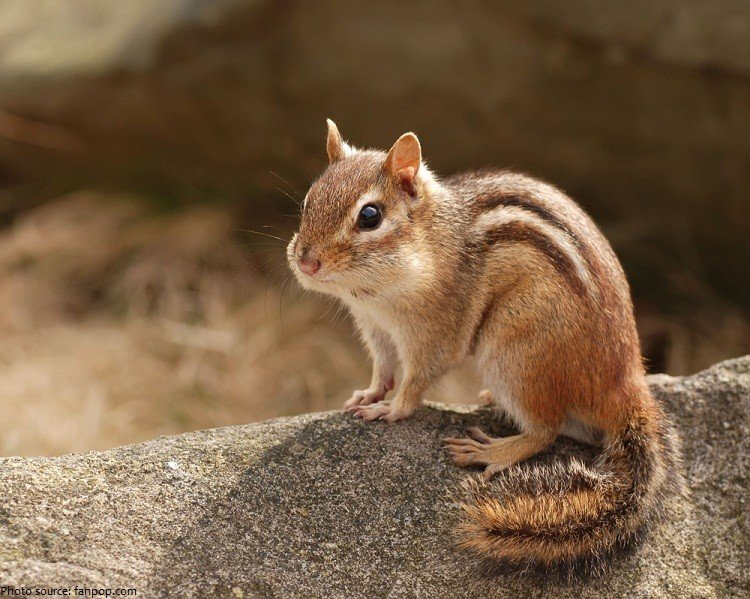
\includegraphics[width=0.5\textwidth]{chipmunk.png}
	\caption{원본 이미지}
\end{figure}

\subsection{흑백 변환}

\begin{lstlisting}
	im = im.convert('L')
	im2 = im.crop((280,150,430,300))
\end{lstlisting}

위 코드에서 원본 이미지를 흑백 변환한 뒤, 특정 구역만 추출하였다.\\

\begin{figure}[ht!]
	\centering
	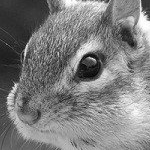
\includegraphics[width=0.5\textwidth]{chipmunk_head.png}
	\caption{흑백 이미지}
\end{figure}


\subsection{이미지 명도 (밝게)}
\begin{lstlisting}
im2_array = np.asarray(im2)
\end{lstlisting}
PIL 이미지에 추가적인 연산을 처리하기 위해서 numpy 배열로 변환해 주었다.\\


\begin{lstlisting}
for x in range(0,150):
	for y in range(0,150):
		im3_array[y,x] = min(im3_array[y,x] + 50, 255)
\end{lstlisting}

흑백 변환된 이미지의 각 픽셀 값을 50씩 더하여 이미지의 밝기를 높여주었다. (최댓값인 255를 넘으면 255로 설정하였다.)\\

\begin{figure}[ht!]
	\centering
	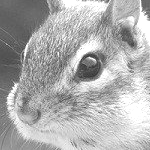
\includegraphics[width=0.5\textwidth]{chipmunk_head_bright.png}
	\caption{밝아진 이미지}
\end{figure}

이미지가 전체적으로 밝아졌다. 하지만 기존에 밝았던 (값이 210 이상인) 부분은 주변 값 보다 픽셀 값 변화가 작기 때문에 선명도가 떨어진 것도 확인할 수 있다. \\

\subsection{이미지 명도 (어둡게)}

\begin{lstlisting}
im4_array = im2_array.copy()
im4_array = im4_array * 0.5
\end{lstlisting}
이번에는 픽셀 값을 반으로 줄여 흑백 이미지를 어둡게 만들어 주었다.\\

\begin{figure}[h]
	\centering
	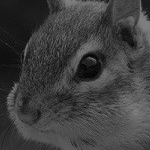
\includegraphics[width=0.5\textwidth]{chipmunk_head_dark.png}
	\caption{어두운 이미지}
\end{figure}

이미지가 전체적으로 어두워졌고 특별한 부분에서 이미지 손실은 없지만, 전체적으로 선명도가 떨어졌다.

\subsection{이미지 생성}

\begin{lstlisting}
grad = np.arange(0,256)
\end{lstlisting}
0에서 255까지 증가하는 256 크기의 배열을 생성하였다.

\begin{lstlisting}
grad = np.tile(grad,[256,1])
\end{lstlisting}
256 크기의 배열을 복제하여 256 x 256 크기의 2차원 배열을 생성하였다.

\begin{figure}[!ht]
	\centering
	
\includegraphics[width=0.5\textwidth]{gradient.png}
	\caption{그라데이션}
\end{figure}

수평으로는 값이 0에서 255까지 증가하는 배열을 사용하였기 때문에 검은색에서 흰색까지 점점 밝아지는 형태를 띠고 있다. 수직으로는 해당 배열을 그대로 복사하였기 때문에 변화가 없다. \\

\section{결론}

\begin{itemize}
\item 이미지 표현
\item 이미지 변환
\item 이미지 손실\\
\end{itemize}

\subsection{이미지 표현}

실습을 진행하면서 python library에 따라 이미지를 다른 방식으로 저장하고 표현하였다. 따라서 원하는 처리를 하기 위해서는 그 처리에 맞는 방식으로 저장하여야 한다.\\

\subsection{이미지 변환}

함수로써의 이미지 변환 처리를 직접 python 라이브러리를 이용하여 구현해 봤다. 흑백 변환, 밝기 조절 등은 쉽게 python 라이브러리를 이용하면 쉽게 처리할 수 있었지만, 픽셀 값 범위 등의 예외 사항을 고려하여 알맞게 처리하여야 한다.\\

\subsection{이미지 변환에 생기는 손실}

이미지를 변환하면서 어쩔 수 없이 이미지 손실이 발생하기도 한다. 예를 들면 이미지를 밝게 만드는 과정에서 픽셀 값이 최댓값을 넘어서는 경우 값을 최댓값으로 설정하여야 한다. 이때 변환된 픽셀이 50을 더하여 최댓값이 된 것인지 그보다 작은 값이 더해진 것인지 구별할 수 없기 때문에 이미지 손실이 생기고 원본 이미지를 복원할 수 없게 된다. 따라서 이미지를 변환할 때 이런 예외 사항과 이미지 손실을 모두 고려하여 처리할 필요가 있다.\\



\end{document}          
